\chapter{PHÂN TÍCH VÀ THIẾT KẾ HỆ THỐNG}


\section{Yêu cầu chức năng và yêu cầu tài nguyên}

Về chức năng, hệ thống cần đọc được bộ trọng số theo định dạng hỗ trợ, dựng đầu vào từ lịch sử hội thoại và sinh câu trả lời. Giao diện nhận nội dung từng phần qua luồng phản hồi, cho phép dừng, xóa lịch sử và đặt lại bộ đệm. Hệ thống hỗ trợ phiên hội thoại để tái sử dụng KV khi tiền tố đầu vào còn phù hợp, đồng thời cung cấp trạng thái bộ nhớ và các chỉ số hiệu năng \cite{moe_tierengine_arch}.

Yêu cầu không hợp lệ, vượt cửa sổ ngữ cảnh hoặc đến khi mô hình đang bận phải nhận thông báo rõ ràng. Với phản hồi dạng luồng, khi người dùng dừng hoặc mất kết nối, tác vụ suy luận kiểm tra tín hiệu hủy tại các điểm đã bố trí và kết thúc để mô hình có thể nhận yêu cầu tiếp theo. Việc hủy có tính hợp tác, không dừng tức thời một phép tính đang chạy. Đường trả lời không theo luồng hiện chưa có cơ chế hủy theo mất kết nối tương đương.

Về tài nguyên, hệ thống không yêu cầu toàn bộ expert phải thường trú trong RAM. Bộ đệm expert có ngân sách tường minh; bộ đệm tái sử dụng, expert đang tính hoặc đang nạp, KV và trọng số chung của mô hình cần được phân biệt khi tính nhu cầu bộ nhớ. Giới hạn bộ đệm expert chỉ kiểm soát một phần tiến trình; cơ chế kiểm tra và bảo vệ RAM được trình bày ở mục 3.7, không phải giới hạn cứng cho tổng bộ nhớ.

Engine chỉ cho một yêu cầu suy luận hoạt động tại một thời điểm. Yêu cầu suy luận mới bị từ chối khi mô hình đang bận; các thao tác theo dõi trạng thái vẫn có thể được phục vụ. Lựa chọn này giúp kiểm soát trạng thái mô hình và phạm vi thực nghiệm, chưa phải thiết kế phục vụ nhiều phiên suy luận đồng thời.

\section{Kiến trúc tổng thể}

Luồng xử lý đi từ giao diện đến lớp HTTP, qua lớp điều phối yêu cầu rồi vào mô hình MoE. Lớp điều phối kiểm tra đầu vào, giới hạn số yêu cầu đang suy luận và chuyển công việc tính toán sang tác vụ riêng để tránh chiếm luồng xử lý bất đồng bộ. Mô hình tổ chức xử lý đầu vào, sinh token, định tuyến expert, quản lý KV và ghi nhận số liệu \cite{moe_tierengine_arch}.

Cùng một mã mô hình phục vụ cả OLMoE và Qwen3; khác biệt về kiến trúc được xử lý bằng cấu hình đọc từ checkpoint. Phần dense có thể chạy trên CPU hoặc GPU qua cuBLAS. Expert INT8 được tính trên CPU bằng Rayon, hoặc trên GPU bằng kernel riêng khi expert đã nằm trong VRAM. Bộ đệm expert trong VRAM và nơi tính expert là hai quyết định tách biệt; mục 3.4 trình bày các tổ hợp được hỗ trợ.


\begin{figure}[htbp]
\centering
\begin{tikzpicture}[box/.append style={text width=3.9cm, minimum height=0.85cm, align=center}]
    \node [box, fill=blue!10] (ui) at (0,0) {Giao diện web};
    \node [box, fill=blue!5] (http) at (5,0) {HTTP và luồng SSE};
    \node [box, fill=orange!10] (engine) at (10,0) {Điều phối yêu cầu\\InferenceEngine};
    \node [box, fill=yellow!15] (model) at (5,-1.65) {Mô hình MoE\\(OLMoE, Qwen3)};
    \node [box, fill=red!10] (guard) at (0,-1.65) {Kiểm tra kế hoạch bộ nhớ\\và bảo vệ RAM};
    \node [box, fill=gray!10] (dense) at (0,-3.55) {Phép chiếu và LM head\\CPU hoặc GPU/cuBLAS};
    \node [box, fill=purple!10] (router) at (5,-3.3) {Router chọn top-$k$};
    \node [box, fill=gray!15] (kv) at (10,-3.3) {Bộ đệm KV và\\tiền tố phiên hội thoại};
    \node [box, fill=purple!20] (expert) at (5,-4.85) {Expert INT8\\CPU (Rayon) / GPU (kernel)};
    \node [box, fill=cyan!10] (ram) at (5,-6.4) {Bộ đệm expert RAM và\\vùng đệm tái sử dụng};
    \node [box, fill=green!10] (vram) at (10,-6.4) {Bộ đệm expert VRAM\\khi bật GPU};
    \node [box, fill=red!10] (file) at (0,-6.4) {Tệp trọng số Safetensors};
    \draw [arrow] (ui) -- (http);
    \draw [arrow] (http) -- (engine);
    \draw [arrow] (engine.south) |- (model.east);
    \draw [arrow] (model) -- (guard);
    \draw [arrow] (model.south west) -- (dense.north east);
    \draw [arrow] (model.south east) -- (kv.north west);
    \draw [arrow] (model) -- (router);
    \draw [arrow] (router) -- (expert);
    \draw [arrow] (ram) -- node[right, font=\footnotesize] {trọng số} (expert);
    \draw [arrow] (file) -- (ram);
    \draw [arrow, <->] (ram) -- (vram);
    \draw [arrow, dashed] (vram.north) -- node[right, font=\footnotesize] {tính tại VRAM} (expert.east);
\end{tikzpicture}
\caption{Kiến trúc tổng thể hệ thống MoE-TierEngine}
\label{fig:system_arch}
\par\smallskip{\footnotesize\RaggedRight Nguồn: nhóm dựng theo mã nguồn \cite{moe_tierengine_arch}. Phần trên thể hiện quan hệ điều phối; các liên kết tệp/RAM/VRAM thể hiện đường cung cấp trọng số. Tác vụ nạp có thể dùng bộ đệm tạm trước khi được giữ trong cache. Hình lược bỏ chi tiết nạp trước và đường trả kết quả; không biểu diễn lịch chạy song song.\par}
\end{figure}


\begin{table}[htbp]
\centering
\setlength{\tabcolsep}{6pt}
\small
\caption{Phân công trách nhiệm các thành phần}
\label{tab:bang_3_1}
\begin{tabularx}{\textwidth}{>{\RaggedRight\arraybackslash}p{4.5cm} >{\RaggedRight\arraybackslash}X}
\toprule
\rowcolor{tableheader}
\textbf{Thành phần} & \textbf{Trách nhiệm} \\
\midrule
HTTP và giao diện & Nhận hội thoại, truyền nội dung qua SSE, hiển thị kết quả và lỗi; xử lý thao tác dừng, xóa lịch sử và đặt lại bộ đệm \\
Lớp điều phối yêu cầu & Kiểm tra đầu vào, chỉ cho một yêu cầu suy luận, chuyển công việc nặng sang tác vụ riêng \\
Mô hình MoE & Nhận diện kiến trúc, mã hóa văn bản, xử lý đầu vào, sinh token, định tuyến, quản lý KV, ghi số liệu và phối hợp các tầng nhớ \\
Expert INT8 & Kiểm tra kích thước và hệ số tỉ lệ, nạp dữ liệu trọng số, tính SwiGLU trên CPU cho một hoặc nhiều token \\
Bộ đọc Safetensors & Tra vị trí, kích thước và kiểu dữ liệu; kiểm phạm vi tệp và đọc trọng số theo nhu cầu \\
Bộ tính toán CPU & Thực hiện các phép chiếu, chuẩn hóa, softmax, attention và các phép toán liên quan \\
Bộ tính toán CUDA & Quản lý ngữ cảnh GPU, cuBLAS, bộ nhớ ghim, vùng cấp phát tái sử dụng, pool expert VRAM và kernel SwiGLU INT8 biên dịch bằng NVRTC \\
Giao diện giám sát & Hiển thị cấu hình, vị trí từng expert trên các tầng, routing của request gần nhất, chia thời gian và bộ nhớ \\
Công cụ thực nghiệm & Ghi cấu hình và mã kiểm tra dữ liệu, gửi bộ yêu cầu thử, lưu kết quả, nhật ký và chuỗi quan sát tài nguyên \\
\bottomrule
\end{tabularx}
\vspace{3pt}\par\noindent\footnotesize\textit{Nguồn: chức năng các thành phần trong mã nguồn \cite{moe_tierengine_arch}. Mô hình nhỏ dùng cho kiểm thử được tách biệt với đường suy luận chính.}
\end{table}

\subsection{Lựa chọn Rust và ranh giới FFI}

Rust được dùng để quản lý quyền sở hữu và kiểm soát việc chia sẻ dữ liệu trong mã an toàn. Các tác vụ CPU và quá trình phục vụ HTTP được tách biệt để tránh một phép tính dài làm nghẽn luồng tiếp nhận yêu cầu.

Phần GPU gọi CUDA và cuBLAS qua giao diện hàm ngoại (FFI). Tại ranh giới này, hệ thống phải kiểm soát ngữ cảnh GPU của luồng, kích thước vùng nhớ, thời gian sống của con trỏ và thứ tự giải phóng tài nguyên. Cơ chế kiểm tra của Rust không tự bảo đảm các điều kiện bên trong thư viện ngoại \cite{moe_tierengine_arch}.

Ví dụ, vùng RAM được ghim để truyền dữ liệu với GPU giữ riêng con trỏ và kích thước cấp phát; dữ liệu được khởi tạo trước khi đường truyền đọc vùng nhớ. Nếu vùng đệm truyền không đủ lớn, hệ thống dùng đường truyền thay thế. Đây là các điều kiện được rà soát cho phần triển khai liên quan, không phải khẳng định toàn bộ mã GPU đã được kiểm chứng an toàn.

\section{Checkpoint và quá trình nạp dữ liệu}

Bộ trọng số được chuẩn bị theo định dạng mà bộ nạp hỗ trợ, gồm các trọng số chung của mô hình và trọng số expert đã lượng tử hóa. Tệp Safetensors cung cấp thông tin về vị trí, kích thước và kiểu dữ liệu của từng mảng trọng số. Dữ liệu một expert ghép ba ma trận cổng, mở rộng và chiếu về chiều ẩn cùng các hệ số tỉ lệ. Bộ đọc kiểm tra tính hợp lệ của kích thước, phép tính dung lượng và phạm vi tệp trước khi cấp phát hoặc đọc dữ liệu.

Khi khởi tạo, hệ thống đọc cấu hình, bộ mã hóa văn bản, khuôn mẫu hội thoại và trọng số chung trong ngân sách tương ứng. Trọng số expert được nạp theo nhu cầu định tuyến hoặc cơ chế nạp trước. Công cụ thực nghiệm lưu mã kiểm tra của bộ trọng số để nhận diện dữ liệu giữa các lượt đo. Việc tính mã này đọc tệp trước khi đo, có thể làm dữ liệu được giữ trong bộ đệm tệp của hệ điều hành. Các thí nghiệm dưới trần RAM xử lý điểm này bằng cách xóa checkpoint khỏi page cache trước mỗi khối đo và kiểm lại bằng công cụ \texttt{fincore}; khi đó mọi lần đọc expert đầu tiên đều đi xuống SSD.

\subsection{Giảm bộ nhớ thường trú cho mô hình lớn}

Với Qwen3-30B-A3B, riêng phần dense đã chiếm 2,46GB ở BF16. Nếu giải nén toàn bộ sang FP32 như cách làm với OLMoE, phần này lên khoảng 4,9GB; riêng bảng embedding $151936\times2048$ ở FP32 đã chiếm khoảng 1,24GB. Engine dùng ba biện pháp để mô hình vừa trong khoảng 6GiB:

\begin{enumerate}
\item \textbf{Dense giữ BF16 trong RAM.} Ma trận attention, router và LM head được giữ nguyên kiểu BF16 của checkpoint và chỉ đổi sang FP32 từng phần trong lúc nhân. Lựa chọn này bật bằng biến môi trường \texttt{MOE\_DENSE\_STORAGE=bf16}.
\item \textbf{Embedding đọc từ tệp.} Mỗi token chỉ cần một hàng của bảng embedding, nên engine đọc đúng hàng đó từ tệp thay vì giữ cả bảng. Chế độ tự động chuyển sang đọc từ tệp khi bảng lớn hơn ngưỡng cấu hình.
\item \textbf{Cache expert có ngân sách theo lớp.} Với 64 MiB/lớp, 48 lớp của Qwen3 dùng 3 GiB cho cache, giữ 14 trong 128 expert mỗi lớp.
\end{enumerate}

Với ba biện pháp này, bộ nhớ ẩn danh của engine khi chạy Qwen3 ổn định ở khoảng 5,7GiB: dense 2,29GiB, cache expert 2,96GiB, còn lại là KV, bộ đệm tính toán và bộ mã hóa văn bản (mục 5.6).

\section{Thiết kế phân tầng expert}

RAM giữ các expert sẵn cho CPU tính. Khi không tìm thấy expert trong RAM, hệ thống kiểm tra bản trong VRAM và truyền về RAM nếu dùng được. Nếu không có bản phù hợp, hệ thống lấy dữ liệu đã nạp trước hoặc đọc tệp trọng số. Tên L1 cho VRAM và L2 cho RAM trên giao diện là cách đặt tên các tầng lưu trữ của engine, khác bộ đệm L1/L2 phần cứng của CPU. Thứ tự tra cứu thực tế bắt đầu từ RAM.


\begin{figure}[htbp]
\centering
\begin{tikzpicture}[box/.append style={text width=3.7cm, minimum height=0.9cm, align=center}, decision/.append style={font=\small, inner sep=1pt}]
    \node [box, fill=blue!10] (start) at (0,0) {Nhận expert từ Router};
    \node [decision] (ram) at (0,-1.25) {Có ở RAM?};
    \node [decision] (vram) at (0,-3.35) {VRAM dùng được?};
    \node [box, fill=yellow!15] (download) at (4.7,-3.35) {Truyền từ GPU về RAM};
    \node [box, fill=red!10] (file) at (-4.7,-3.35) {Lấy bản đã nạp trước;\\nếu chưa có thì đọc tệp};
    \node [box, fill=purple!10] (compute) at (0,-5.25) {Tính expert trên CPU};
    \node [box, fill=cyan!10, text width=8.7cm, minimum height=1.4cm] (admit) at (0,-7.25) {Sau khi tính: xét lưu lại expert trong RAM.\\Nếu cần chỗ, loại expert cũ và thử giữ expert cũ ở VRAM trước khi tái sử dụng vùng đệm.\\Nếu GPU đang bật, bỏ bản VRAM tương ứng khi giữ expert vừa dùng trong RAM.};
    \draw [arrow] (start) -- (ram);
    \draw [arrow] (ram) -- node[right] {Không} (vram);
    \draw [arrow] (ram.west) -- node[above] {Có} (-7,-1.25) |- (compute.west);
    \draw [arrow] (vram) -- node[above] {Có} (download);
    \draw [arrow] (vram) -- node[above, pos=0.2, font=\footnotesize] {Không} (file);
    \draw [arrow] (download.south) |- (compute.east);
    \draw [arrow] (file.south) |- (compute.west);
    \draw [arrow] (compute) -- (admit);
\end{tikzpicture}
\caption{Truy xuất và lưu lại expert theo chính sách victim}
\label{fig:tiering_victim}
\par\smallskip{\footnotesize\RaggedRight Nguồn: các đường lấy, tính và lưu lại expert trong mã nguồn \cite{moe_tierengine_arch}. Hình lược bỏ lịch nạp trước và chi tiết xử lý lỗi. Truyền từ VRAM thất bại thì có thể dùng bản đã nạp trước hoặc đọc tệp. Nếu expert không vừa ngân sách RAM, hệ thống không giữ trong cache RAM và có thể thử giữ ở VRAM. Mọi đường VRAM phụ thuộc GPU được bật và tài nguyên khả dụng.\par}
\end{figure}


Chính sách victim ưu tiên dùng VRAM giữ expert bị loại khỏi RAM để giảm bản sao trùng giữa hai tầng. Khi GPU đang bật và expert được giữ lại trong RAM sau khi tính, bản tương ứng trong VRAM được bỏ; thao tác này diễn ra sau khi truyền dữ liệu về RAM đã hoàn tất. Chính sách inclusive được giữ làm đối chứng. Hai chính sách thay đổi nơi lưu trữ, không thay trọng số mô hình hoặc thứ tự tổng hợp đầu ra expert.

\subsection{Ba chế độ sử dụng GPU}

GPU được điều khiển bằng ba công tắc độc lập, đọc khi khởi động. Bảng~\ref{tab:gpu_modes} mô tả các tổ hợp được dùng trong thực nghiệm.

\begin{table}[htbp]
\centering
\caption{Các chế độ sử dụng GPU}
\label{tab:gpu_modes}
\small
\setlength{\tabcolsep}{3pt}
\begin{tabularx}{\textwidth}{>{\RaggedRight\arraybackslash}p{2.6cm} >{\RaggedRight\arraybackslash\footnotesize}p{5.0cm} >{\RaggedRight\arraybackslash}X}
\toprule
\textbf{Chế độ} & \textbf{Biến môi trường} & \textbf{Dữ liệu trên VRAM và luồng tính} \\
\midrule
CPU & \texttt{MOE\_GPU\_MODE=cpu} & Không dùng GPU. Dense và expert tính trên CPU. \\
Dense trên GPU & \texttt{MOE\_GPU\_MODE=auto} & Dense FP32 trên VRAM, tính bằng cuBLAS. Expert tính trên CPU. \\
Tầng VRAM expert & thêm \texttt{MOE\_GPU\_EXPERT\_TIER=on} & VRAM giữ thêm expert theo chính sách victim. Expert lấy từ VRAM được chép về RAM để CPU tính. \\
Tính expert trên GPU & thêm \texttt{MOE\_GPU\_EXPERT\_COMPUTE=on} & Pool VRAM lấp đầy một lần rồi giữ cố định. Expert có trong pool được tính bằng kernel trên GPU; expert ngoài pool vẫn đi qua RAM và CPU. \\
VRAM chỉ chứa expert & thêm \texttt{MOE\_GPU\_DENSE=off} và \texttt{MOE\_GPU\_EXPERT\_PLACEMENT} & Dense ở lại CPU. Toàn bộ VRAM dành cho pool expert, nạp sẵn lúc khởi động theo hồ sơ tần suất (mục 4.5). Expert trong pool tính trên GPU như dòng trên. \\
\bottomrule
\end{tabularx}
\par\smallskip{\footnotesize\RaggedRight Nguồn: cấu hình GPU trong mã nguồn \cite{moe_tierengine_arch}.\par}
\end{table}

Khi khởi động, engine ước lượng dung lượng VRAM cần cho dense và vùng tính tạm. Nếu không đủ, engine tự chuyển sang chế độ CPU và ghi lý do vào nhật ký thay vì dừng với lỗi. Trường hợp này xảy ra với Qwen3 trên GTX 1650 4GB, vì dense FP32 của Qwen3 cần khoảng 4,9GB VRAM. Ở bản đầu, pool expert được cấp phát trong cùng khối với dense, nên khi dense không lên GPU được thì pool cũng không được bật. Bản hiện tại tách hai quyết định này: với \texttt{MOE\_GPU\_DENSE=off}, engine bỏ qua việc đưa dense lên GPU nhưng vẫn tạo pool expert và kernel tính expert, mọi phép chiếu dense đi theo đường CPU. Kernel expert nhận đầu vào và trả kết quả qua RAM (mục 4.5), nên không cần dense nằm trên GPU. Mặc định vẫn đưa dense lên GPU như trước; chế độ mới phải bật tường minh.

\section{Quản lý bộ nhớ và session}

\begin{table}[htbp]
\centering
\setlength{\tabcolsep}{6pt}
\small
\caption{Các vùng bộ nhớ cần phân biệt}
\label{tab:bang_3_2}
\begin{tabularx}{\textwidth}{>{\RaggedRight\arraybackslash}p{4.0cm} >{\RaggedRight\arraybackslash}p{4.5cm} >{\RaggedRight\arraybackslash}X}
\toprule
\rowcolor{tableheader}
\textbf{Vùng} & \textbf{Vai trò} & \textbf{Giới hạn cần ghi nhận} \\
\midrule
Trọng số chung trong RAM & Phục vụ CPU hoặc đường tính thay thế & Không tự được giải phóng khi bật GPU \\
Trọng số chung trong VRAM & Phục vụ các phép chiếu trên GPU & Cùng dùng VRAM với bộ đệm expert và vùng tính tạm \\
Bộ đệm expert RAM và vùng tái sử dụng & Giữ dữ liệu expert và vùng đệm đã cấp phát & Cùng tính dung lượng cấp phát vào ngân sách mỗi lớp \\
Expert đang dùng hoặc đang nạp & Dữ liệu phục vụ tính toán và nạp trước & Cần dự phòng riêng ngoài dữ liệu giữ trong cache \\
KV và phiên hội thoại & Giữ khóa, giá trị, mã token và trạng thái dùng lại & Dữ liệu hợp lệ khác dung lượng cấp phát và phần quản lý \\
Vùng tính tạm, bộ nhớ ghim và vùng tái sử dụng GPU & Phục vụ tính toán, truyền dữ liệu và tái sử dụng & Số liệu hệ thống báo có thể chưa bao hết cấp phát thực \\
Bộ mã hóa, bộ cấp phát và môi trường thực thi & Các thành phần hỗ trợ tiến trình & Không nằm trọn trong ngân sách bộ đệm \\
\bottomrule
\end{tabularx}
\vspace{3pt}\par\noindent\footnotesize\textit{Nguồn: thiết kế và giới hạn accounting hiện hành \cite{moe_tierengine_arch}, \cite{exp_prefill_i5}.}
\end{table}

Bộ đệm expert và vùng đệm tái sử dụng cùng tính vào ngân sách dung lượng cấp phát của mỗi lớp. Kế hoạch bộ nhớ còn dự phòng dữ liệu expert đang dùng hoặc đang nạp theo mức $(k+2)B_e$, trong đó $k$ là số expert được chọn và $B_e$ là dung lượng dữ liệu của một expert. Mức dự phòng này chưa gồm dữ liệu quản lý và các vùng khác, không phải giới hạn cứng cho tổng cấp phát. Khi xử lý đầu vào, nhóm nạp trước được giới hạn tối đa $k$ expert; expert còn lại được đọc khi cần.

Ngân sách lưu phiên hội thoại tính dung lượng đã cấp phát cho các mảng khóa, giá trị, mã token và một phần dữ liệu quản lý. Phần quản lý bảng băm, bộ cấp phát và KV của yêu cầu đang chạy vẫn cần được xét riêng. Đặt lại bộ đệm xóa các mục đã lưu và vùng đệm tái sử dụng, nhưng giữ cấu hình ngân sách để phiên sau tiếp tục lưu KV. RSS không nhất thiết giảm ngay sau thao tác này, vì bộ cấp phát có thể giữ lại trang nhớ.

\section{HTTP/SSE, hủy yêu cầu và tính nhất quán giao diện}


\begin{figure}[htbp]
\centering
\begin{tikzpicture}[node distance=1.0cm, auto]
    \node [box, fill=blue!10] (user) {Client (Web / Runner)};
    \node [box, fill=orange!10, right=2.5cm of user] (http) {HTTP Facade};
    \node [box, fill=purple!10, right=2.5cm of http] (worker) {Blocking Worker};

    \node [below=5.0cm of user] (u_end) {};
    \node [below=5.0cm of http] (h_end) {};
    \node [below=5.0cm of worker] (w_end) {};

    \draw [dashed] (user) -- (u_end);
    \draw [dashed] (http) -- (h_end);
    \draw [dashed] (worker) -- (w_end);

    % Message sequence
    \draw [arrow] ($(user.south)+(0,-0.4)$) -- node [above, scale=0.8] {POST (messages, session)} ($(http.south)+(0,-0.4)$);
    \draw [arrow] ($(http.south)+(0,-0.9)$) -- node [above, scale=0.8] {Acquire gate, spawn task} ($(worker.south)+(0,-0.9)$);
    \draw [arrow] ($(worker.south)+(0,-1.5)$) -- node [above, scale=0.8] {Worker ready (preflight OK)} ($(http.south)+(0,-1.5)$);
    \draw [arrow] ($(http.south)+(0,-2.0)$) -- node [above, scale=0.8] {SSE Stream Header (200 OK)} ($(user.south)+(0,-2.0)$);
    \draw [arrow] ($(worker.south)+(0,-2.6)$) -- node [above, scale=0.8] {Delta token chunks} ($(http.south)+(0,-2.6)$);
    \draw [arrow] ($(http.south)+(0,-3.1)$) -- node [above, scale=0.8] {Content chunk (SSE)} ($(user.south)+(0,-3.1)$);
    \draw [arrow] ($(worker.south)+(0,-3.7)$) -- node [above, scale=0.8] {Finished / Terminal status} ($(http.south)+(0,-3.7)$);
    \draw [arrow] ($(http.south)+(0,-4.1)$) -- node [above, scale=0.8] {Terminal result (SSE)} ($(user.south)+(0,-4.1)$);
    \draw [arrow] ($(http.south)+(0,-4.6)$) -- node [above, scale=0.8] {data: [DONE]} ($(user.south)+(0,-4.6)$);
\end{tikzpicture}
\caption{Vòng đời xử lý yêu cầu suy luận streaming qua HTTP/SSE}
\label{fig:streaming_lifecycle}
\par\smallskip{\footnotesize\RaggedRight Nguồn: nhóm dựng theo HTTP handler và blocking worker \cite{moe_tierengine_arch}. Endpoint: \nolinkurl{/v1/chat/completions}. Hình mô tả luồng thành công, lược bỏ nhánh lỗi và hủy.\par}
\end{figure}


Công việc suy luận chạy trong tác vụ tính toán riêng, tránh chiếm luồng xử lý bất đồng bộ bằng phép tính dài. Hàng đợi truyền kết quả có giới hạn; nếu phía nhận không đọc trong thời gian cho phép, tác vụ kết thúc với lỗi. Cơ chế giới hạn truy cập từ chối yêu cầu suy luận mới khi mô hình đang bận.

Trước khi SSE bắt đầu, hệ thống có thể trả lỗi bằng mã trạng thái HTTP. Sau khi phần đầu phản hồi đã gửi, lỗi được thông báo trong luồng dữ liệu. Giao diện chỉ lưu câu trả lời hoàn tất khi nhận đủ thông tin kết quả cuối, dấu kết thúc và kết thúc luồng hợp lệ. Nội dung bị dừng hoặc mất kết nối không được ghi thành câu trả lời hoàn chỉnh. Đường trả lời không theo luồng chưa có cơ chế hủy theo mất kết nối tương đương.

\section{Preflight và bảo vệ RAM hợp tác}

Trước khi nạp trọng số lớn, hệ thống ước lượng nhu cầu gồm trọng số dense theo kiểu lưu đã chọn, bộ đệm theo cấu hình, dự phòng phiên hội thoại, yêu cầu đang chạy và phần phụ trợ. Hệ thống từ chối nếu kế hoạch vượt giới hạn tiến trình hoặc không chừa đủ RAM cho hệ thống. Trong khi sinh, cơ chế bảo vệ kiểm tra RSS và RAM có thể cấp phát tại các điểm kiểm tra hủy. Việc đọc thống kê bộ nhớ được giãn cách tối thiểu 25 ms; đây không phải bộ lấy mẫu chạy liên tục đúng mỗi 25 ms.

Ngưỡng RSS mặc định bằng một nửa RAM máy, tối đa 6 GiB, và có thể đặt lại bằng \texttt{MOE\_RAM\_LIMIT\_BYTES}; mức RAM cần chừa cho hệ thống mặc định là 1 GiB. Với Qwen3, ngưỡng được đặt 9 GiB. Ví dụ, cấu hình cache 128 MiB/lớp cho Qwen3 bị từ chối ngay khi khởi động vì phần dự trữ ước lượng 9,94GB vượt ngưỡng 9 GiB; tiến trình dừng với thông báo rõ ràng thay vì bị hệ điều hành dừng giữa chừng. Khi phát hiện áp lực bộ nhớ, cơ chế bảo vệ trả lỗi thiếu bộ nhớ. Trước khi mở luồng SSE, lỗi có thể được trả bằng HTTP 503; sau khi luồng đã được chấp nhận, lỗi được gửi qua sự kiện trong luồng. Khi tác vụ dừng sử dụng dữ liệu, hệ thống xóa bộ đệm expert RAM, phiên hội thoại và vùng đệm tái sử dụng theo đường xử lý lỗi. Trọng số chung và bộ đệm VRAM có thể còn được giữ; bộ cấp phát không được bảo đảm trả trang nhớ ngay cho hệ điều hành.

Đây là bảo vệ hợp tác, không phải cơ chế của hệ điều hành ngăn mọi cấp phát vượt ngưỡng. Bộ nhớ có thể tăng giữa các điểm kiểm tra; hoạt động của trình điều khiển và thư viện cũng có thể tạo thêm cấp phát. Việc đọc thống kê Linux và giới hạn nhóm tiến trình cgroup v2 chỉ bao phủ phần hệ thống quan sát được. Khi thực nghiệm, nhóm còn dùng bộ giám sát độc lập, vì trạng thái do máy chủ trả về có thể là bản ghi trước đó khi mô hình đang bận.

Để kiểm chứng engine thực sự chạy được trong một lượng RAM cho trước, công cụ thực nghiệm đặt engine vào một cgroup v2 riêng với \texttt{memory.max} bằng trần cần thử và \texttt{memory.swap.max} bằng 0 \cite{linux_cgroup_v2}. Trần này do nhân Linux áp đặt và tính cả page cache của tệp checkpoint. Nếu engine vượt trần, nhân hệ điều hành sẽ thu hồi page cache rồi dừng tiến trình; số lần dừng như vậy được đọc lại từ bộ đếm \texttt{oom\_kill} của cgroup. Ngưỡng của RAM guard được đặt thấp hơn trần cgroup 1 GiB, để engine từ chối yêu cầu trước khi nhân hệ điều hành phải can thiệp.

\section{Giao diện giám sát}

Giao diện web vừa là nơi hội thoại, vừa là công cụ quan sát hệ thống. Mọi số liệu hiển thị đều lấy từ API của engine, gồm dữ liệu trả về sau mỗi request và trạng thái expert theo từng lớp; giao diện không chứa số liệu minh họa hay giá trị viết sẵn.

\begin{figure}[htbp]
\centering
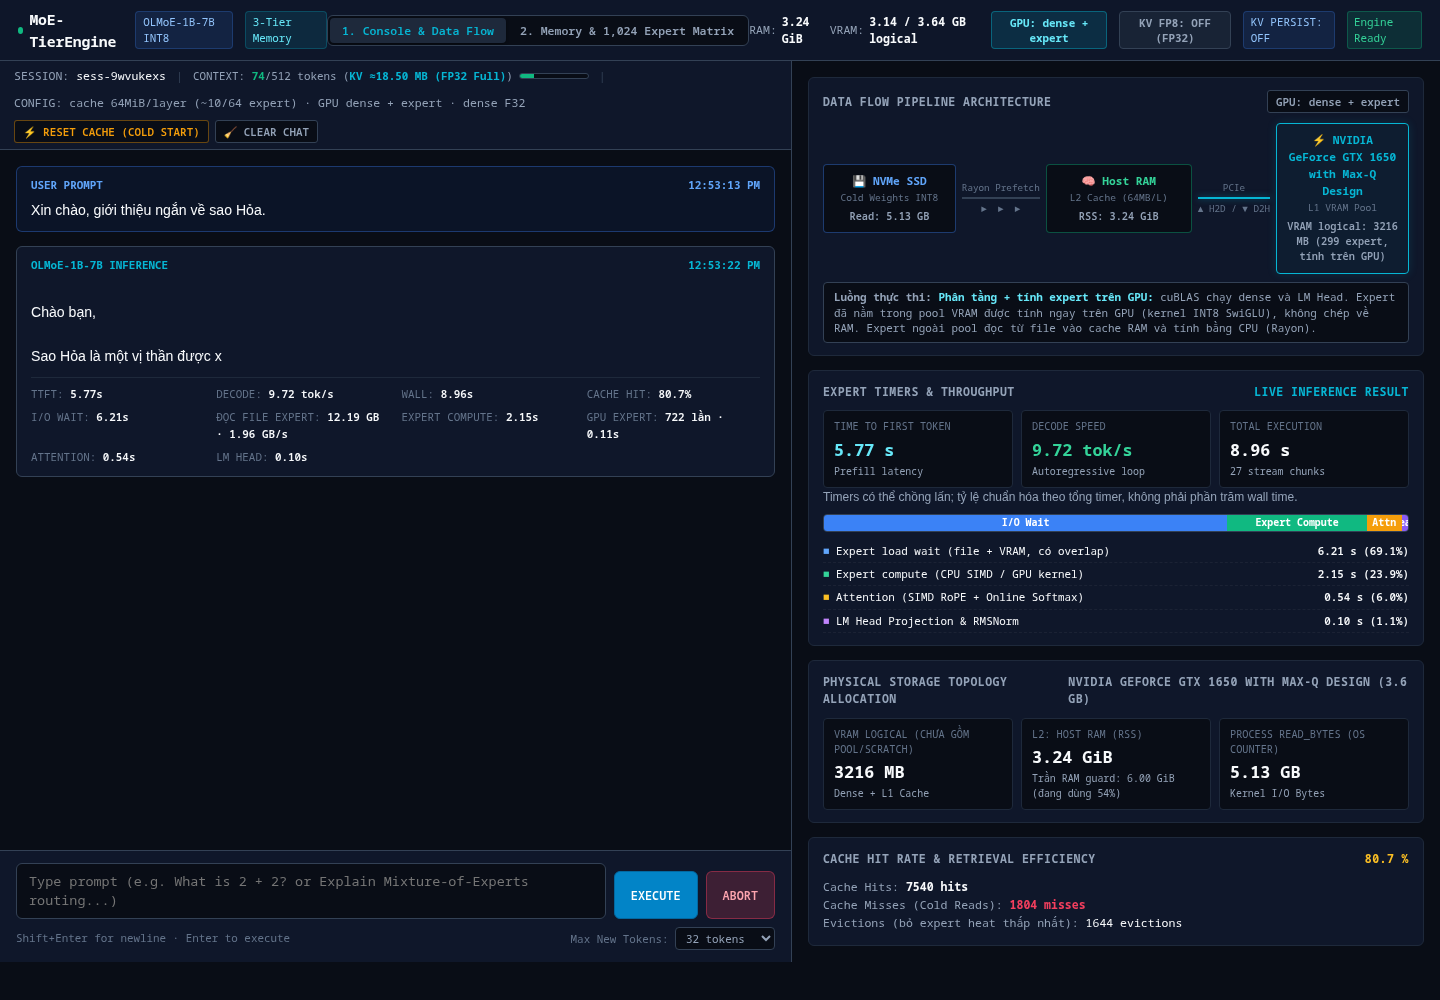
\includegraphics[width=\textwidth]{images/web_olmoe_gpu.png}
\caption{Giao diện hội thoại và bảng số liệu của một request}
\label{fig:web_console}
\par\smallskip{\footnotesize\RaggedRight Nguồn: ảnh chụp giao diện khi chạy OLMoE-1B-7B ở chế độ tính expert trên GPU, máy i5. Một request 32 token; số liệu là của request này, không phải kết quả đo chính thức.\par}
\end{figure}

Trang thứ nhất (Hình~\ref{fig:web_console}) hiển thị dòng cấu hình (ngân sách cache, chế độ GPU, kiểu lưu dense), câu trả lời và các chỉ số của từng request: TTFT, tốc độ sinh, chia thời gian giữa chờ expert, tính expert, attention và LM head, lượng dữ liệu đọc tệp cùng tốc độ đọc. Bảng bộ nhớ hiển thị RSS cùng trần RAM của engine; bảng cache hiển thị số lần tìm thấy, không tìm thấy và số expert bị loại.

\begin{figure}[htbp]
\centering
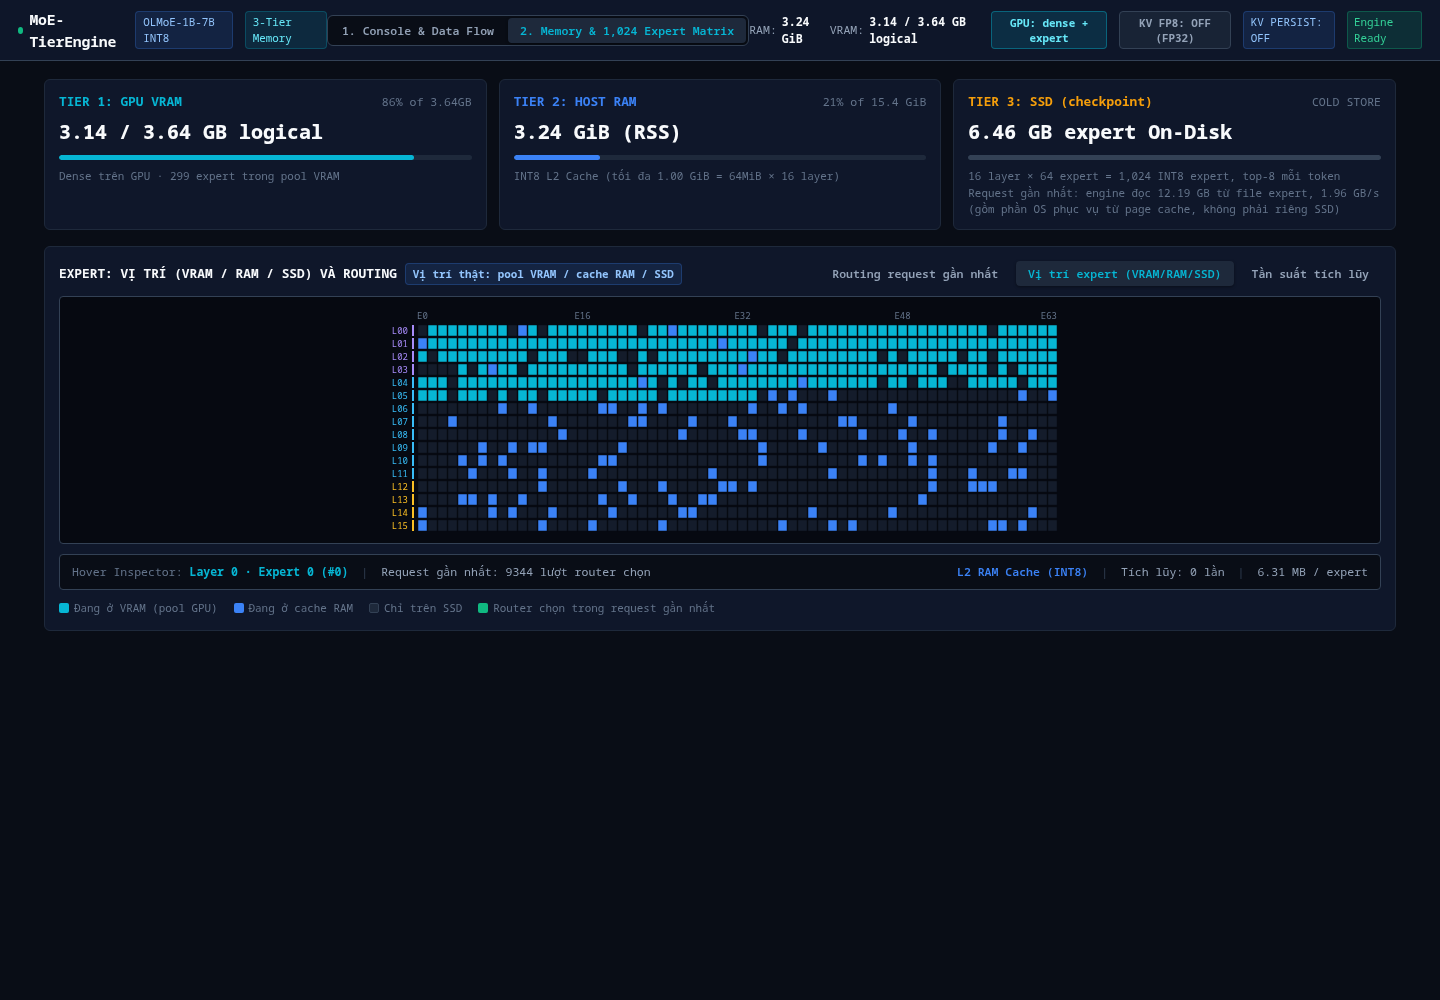
\includegraphics[width=\textwidth]{images/web_olmoe_matrix.png}
\caption{Ma trận vị trí expert theo lớp}
\label{fig:web_matrix}
\par\smallskip{\footnotesize\RaggedRight Nguồn: ảnh chụp cùng phiên với Hình~\ref{fig:web_console}. Mỗi ô là một expert; màu thể hiện expert đang nằm trong VRAM, trong RAM hay chưa nạp.\par}
\end{figure}

Trang thứ hai (Hình~\ref{fig:web_matrix}) vẽ ma trận $L\times E$ expert, tự điều chỉnh theo mô hình đang chạy. Chế độ vị trí vật lý tô từng ô theo nơi expert đang nằm, lấy từ danh sách expert của pool VRAM và cache RAM. Chế độ routing tô các expert được Router chọn trong request gần nhất, tính bằng hiệu bộ đếm sử dụng trước và sau request. Chế độ tần suất hiển thị mức sử dụng tích lũy. Trên ma trận của OLMoE ở chế độ tính expert trên GPU có thể thấy pool VRAM tập trung ở các lớp đầu, đúng với chính sách lấp đầy theo thứ tự nạp.

Để chạy các cấu hình một cách ổn định, kho mã có script \texttt{tools/demo.sh} với bốn cấu hình đặt sẵn: OLMoE trên GPU, OLMoE trên CPU, Qwen3 trên CPU và Qwen3 với GPU. Cấu hình Qwen3 với GPU dùng đúng cấu hình đã đo ở mục 5.7: dense trên CPU, VRAM chỉ chứa expert nạp sẵn theo hồ sơ tần suất, chạy được trên cả GPU 4GB và 8GB. Giao diện ghi rõ chế độ này là ``GPU: expert (dense CPU). Script luôn build lại binary trước khi chạy, vì giao diện được nhúng vào binary.
